\subsubsection{Image Analysis Techniques}
	There are a number of analysis techniques which can be applied to imagery to extract information. Perhaps the most common is analysing the pixels in an image to identify discontinuities in their data values which suggests the edge of an object, structure or land mass. Such functionality is readily available on desktop image processing packages designed for amateur photographers \citep{photoshop}. But scientific and engineering applications of edge detection provide far great levels of sensitivity helping isolate objects that can be subsequently measured with high level of accuracy \citep{matlabedge}.
	\paragraph{Thresholding}
		Image thresholding is the most basic form of image segmentation \citep{haralock1991computer}. At its simplest this would entail taking a greyscale image, examining the intensity of each pixel and setting those below a certain threshold to black and those above it to white as shown in Figure \ref{fig:threshold} below. By thresholding an image, objects lose detail but their silhouettes become clearer making them more visible to object detection techniques.
		\begin{figure}[h!]
			\centering
			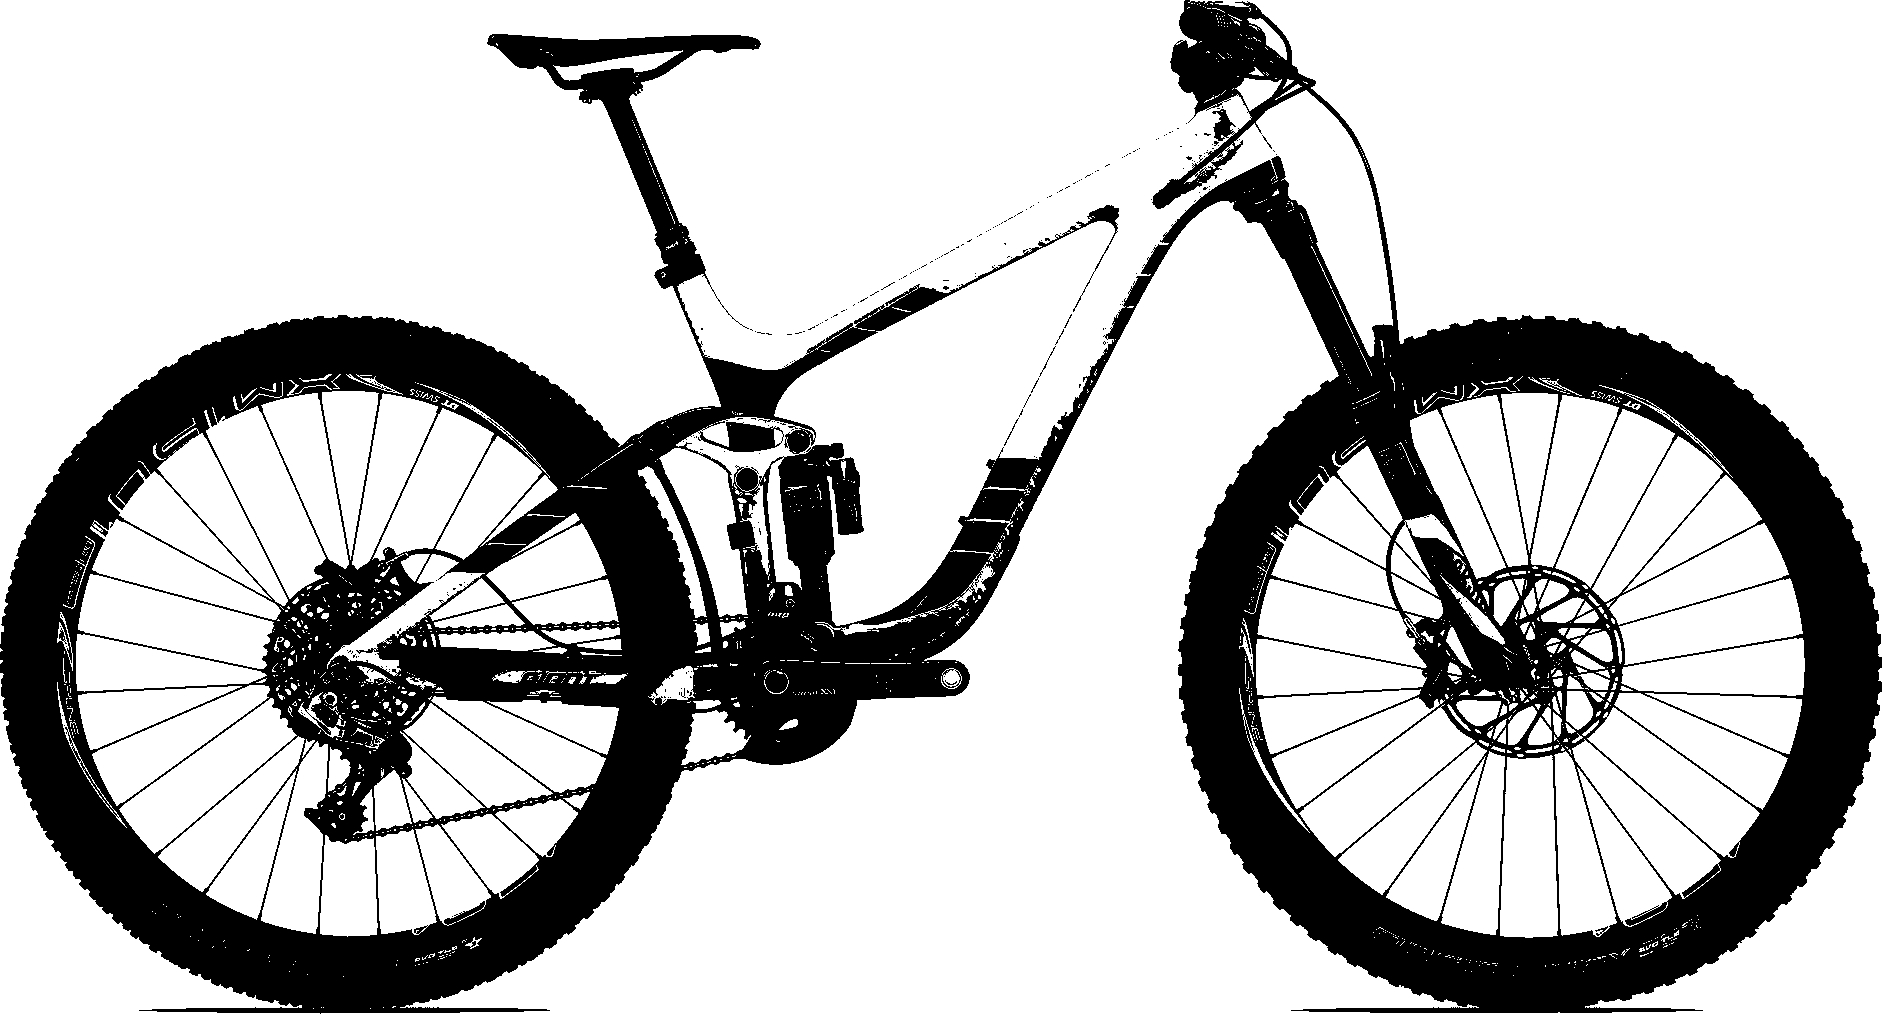
\includegraphics[width=8cm]{../images/reign_threshold.jpg}
			\caption{A copy of Figure \ref{fig:fsandht} with thresholding applied}
			\label{fig:threshold}
		\end{figure}
	\paragraph{Edge Detection}
	This is the application of mathematical algorithms to locate and highlight the edges of features in an image. There are multiple algorithms which can be used for edge detection, including Sobel, Roberts, Canny, and fuzzy logic, although all utilise the same basic concept of comparing the data values of adjacent pixels to find discontinuities from one value to another.
	\begin{table}[h!]
		\centering
		\caption{Table of pixel data showing an edge}
		\label{tab:edgePixels}
		\begin{tabular}{|c|c|c|c|c|c|c|}
			\hline
			5&7&6&4&152&148&149\\
			\hline
			\cellcolor[HTML]{0D0D0D}&
			\cellcolor[HTML]{121212}&
			\cellcolor[HTML]{0F0F0F}&
			\cellcolor[HTML]{0a0a0a}&
			\cellcolor[HTML]{989898}&
			\cellcolor[HTML]{949494}&
			\cellcolor[HTML]{959595}\\
			\hline
		\end{tabular}
	\end{table}\\
	Table \ref{tab:edgePixels} represents possible pixel values of an edge indicated by the large difference between 4 and 152. The applied algorithm will pick up this discontinuity which will be highlighted on the resulting image. A common application for edge detection is text recognition such as in automatic number plate recognition (ANPR) \citep{anpr} where unwanted background data is automatically excluded using thresholding techniques to highlight the block shapes of the vehicle registration plate. Figure \ref{fig:anpr} shows an image which has had edge detection applied with the number plate of the car clearly visible.
	\begin{figure}[h!]
		\centering
		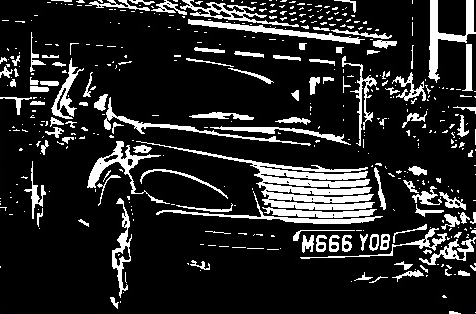
\includegraphics[width=10cm]{../images/anpr.jpg}
		\caption{Edge detection applied to an image for number plate recognition}
		\label{fig:anpr}
	\end{figure} 
	\paragraph{Hough Transform}\label{sec:lit_review_hough}\todo{complete hough transform section}
	Originally created in 1962 by Paul Hough, the Hough transform methods offer techniques for the discovery of imperfect objects in images. The original algorithms were created for the detection of lines but have since been improved and adapted to find circles, ellipses, and other basic shapes. 
	\\\\
	While edge detection is suitable for highlighting critical points in an image, it can be problematic if the base image is not well lit or sharply focussed causing an edge detector to produce imperfect lines. Such artefacts can make rudimentary feature detection techniques difficult but the Hough Transformation techniques circumvent such issues by considering points as a part of an object through a voting procedure.
	\subparagraph{Linear Hough Transform}
	To locate straight lines in an image, the linear Hough transform utilises Hesse normal form $r = x cos \theta + y sin \theta$. Lines, or planes, in an image are expressed as pairs of $(r, \theta)$ 
	\subparagraph{Circular Hough Transform}
	
	\paragraph{Taking Measurements}\label{sec:taking_measurements}
		To measure the dimensions of an object in an image, certain data about the camera and its location are required. By using digital imagery, the majority of this information is automatically provided as each image contains metadata or EXchangeable Image Format (EXIF) data which includes information such as camera manufacturer, focal length, image size, and location if available.
	\begin{equation}
		\label{equ:measureobj}
		H_{o} = \Bigg(\frac{f\times\big(\frac{H_{i}}{H_{s}}\big)}{D - f}\Bigg)\times H_{c}
	\end{equation}
	\begin{where}
		\item $f$~~~~is the focal length of the camera lens
		\item $D$~~~is the distance to the object
		\item $H_{o}$~~is the height of the object
		\item $H_{i}$~~is the height of the image in pixels
		\item $H_{s}$~~is the height of the camera sensor
		\item $H_{c}$~~is the height of the camera from the ground
	\end{where}
	\vspace{5mm}
	The process to calculate the height of an object in an image is shown in Equation \ref{equ:measureobj}. Necessary data, such as $f$, $H_i$, and $H_s$ can be acquired from EXIF data. However $D$ and $H_c$ are not collected by the camera and must be measured. When dealing with image analysis this means that this data has to be collected at the time the image is taken.
	\\\\
	However it is not necessary to collect data for $H_o$ - the distance of the object being measured from the ground - as the size of the object is in direct proportion to its size on the camera’s sensor so is not required. To test this equation, data was created from known object heights which was then re-used to see if the calculated height was equal to the actual height. For example:\todo{What is going on here?}
	\\\\
	To circumvent the need to collect data for $H_c$ - the height of the camera -, a reference object of a known size can be included in the image as this allows a comparison to be made between the height of the object to be measured and the reference object. The previously mentioned Mars rover, Curiosity, carries a United States penny as a reference object so that its cameras can be precisely calibrated using reference charts as shown in Figure \ref{fig:curiosity_calibration_chart}.
	\begin{figure}[h!]
		\centering
		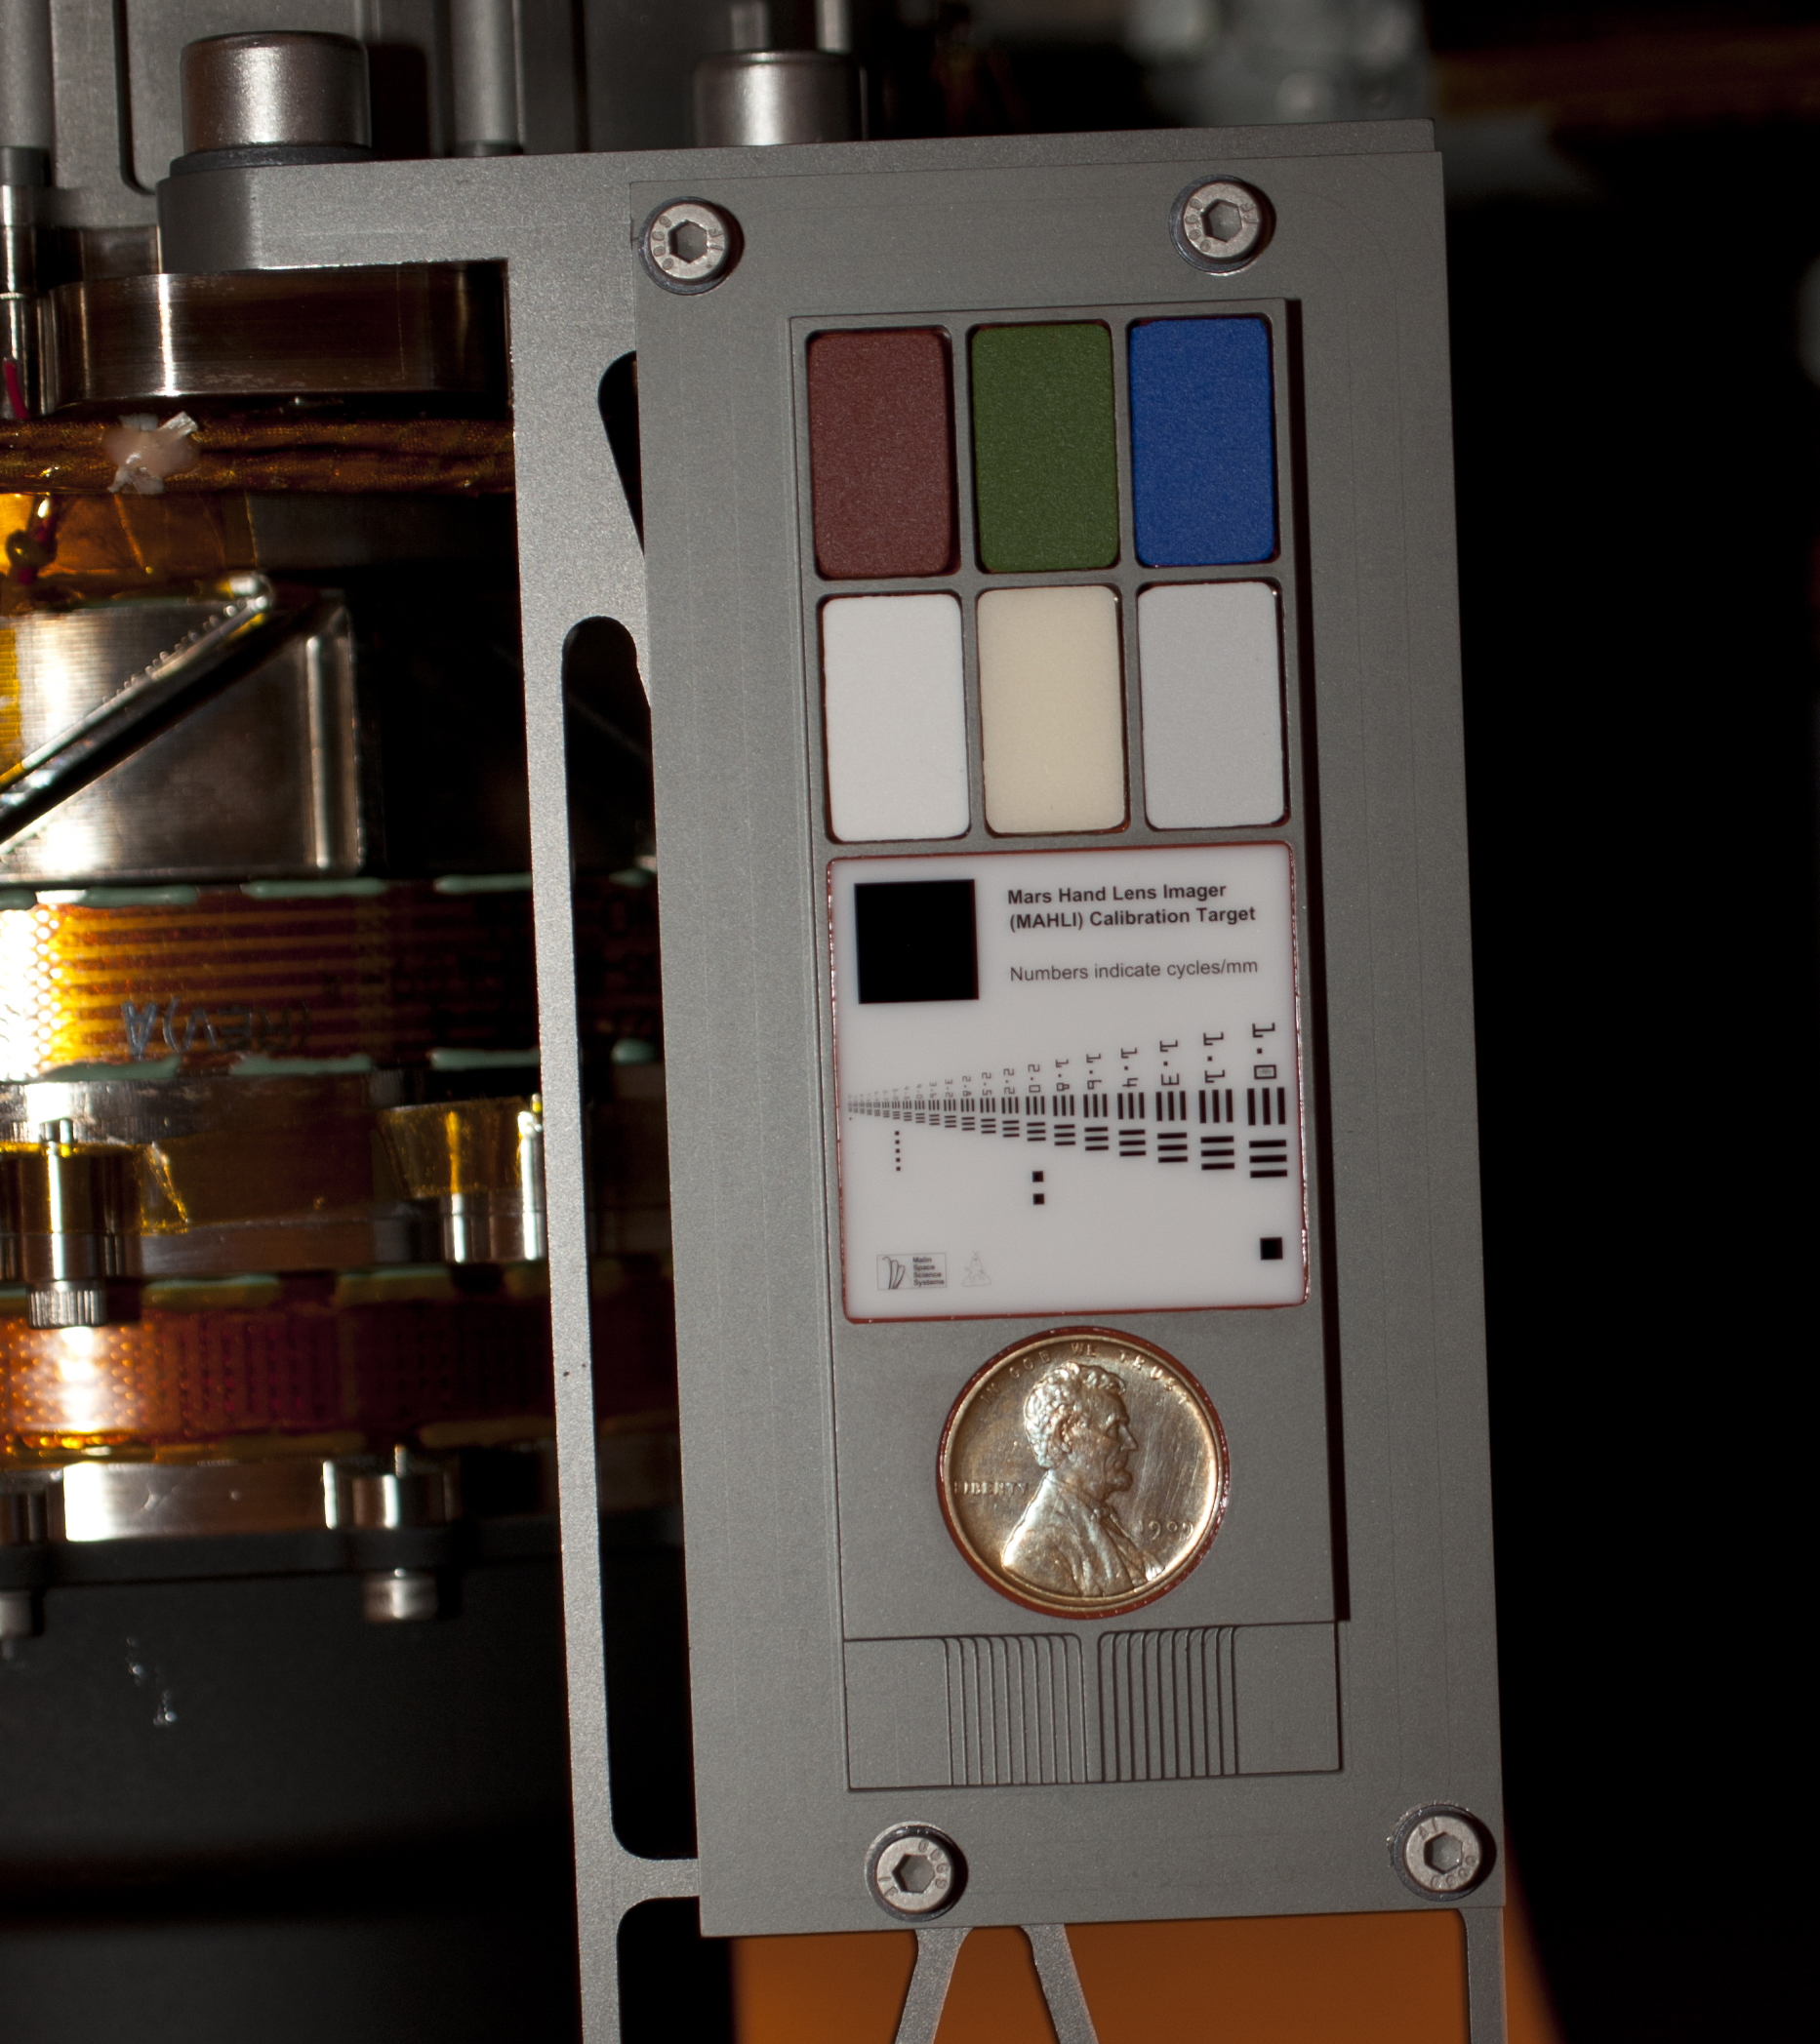
\includegraphics[width=7cm]{../images/curiosity_calibration_chart.jpg}
		\caption{Contact Instrument Calibration Targets on Mars Rover Curiosity \citep{curiosity_image_calibration}}
		\label{fig:curiosity_calibration_chart}
	\end{figure}\\
	However, the reference object must be located in the image using a technique such as \todo{Add section or briefly explain} BLOB analysis or Hough transforms. Once the object is found, its width or height in pixels in the image is collected and compared against its actual size to give a ratio for applying to the pixel count of the object to calculate its real world height. For example, if a reference object that is 2mm wide measures 200 pixels across in an image then it can be concluded that 100 pixels in the image corresponds to 1mm in the real world. Knowing this ratio, any other objects that can be measured in pixels can have the real world measurement estimated as long as they are approximately the same distance from the camera as the reference object.
	\\\\
	This process will be applied during this project in some manner. Either a reference object will be used or measurements for $H_c$ (the height of the camera from the ground) will be taken at the time the image is captured as knowing these measurements is vital to achieving reliable results that will ensure that suspension units are correctly configured as previously discussed. But while incorporating Equation \ref{equ:measureobj} in an application will be relatively simple, collecting the necessary data without too much user interaction may be more difficult.